\begin{figure}[H]
\centering
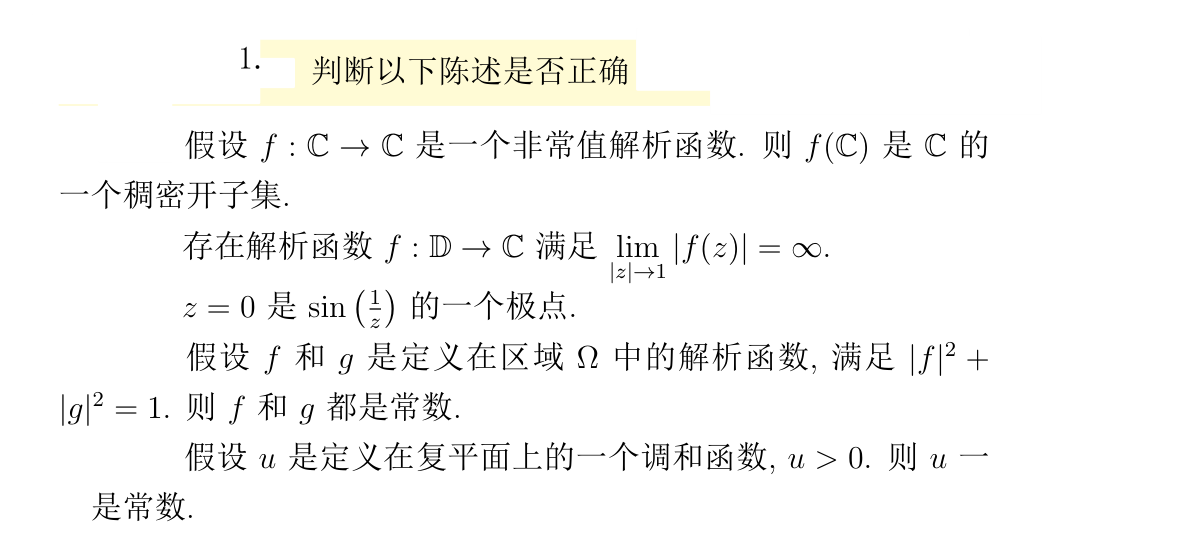
\includegraphics[width=\textwidth]{2-复变函数期末附加题-2025062122.png}
% \caption{}
\label{}
\end{figure}

\begin{enumerate}
	\item 对. 反证而设 $w\not\in \overline{f(\mathbb{C})}^{\mathbb{C}}$, 则存在 $r>0$,使得 $\lvert f (z)-w \rvert\geq r,\forall z\in \mathbb{C}$. 定义 $g=\frac{1}{f-w}$,于是 $\lvert g \rvert\leq\frac{1}{r}$ 为有界整函数,故 $g\equiv c$,$f\equiv c'$. 矛盾!
	\item 错,显然 $f$ 只可能在 $\mathbb{D}$ 内有有限零点,除掉 Blaschke 乘积,得到 $\mathbb{D}$ 上无零点解析函数 $g\coloneqq f/B$,补充 $\left.g\right|_{\partial \mathbb{D}}=0$,故 $g$ 在 $\overline{\mathbb{D}}$ 连续,在 $\mathbb{D}$ 解析. 利用最大模原理 $\left\lvert  \frac{1}{g}  \right\rvert\leq\frac{1}{\infty}=0$,故 $g$ 无定义. 矛盾!
	\item 错. 考虑洛朗展开 $\sin\left( \frac{1}{z} \right)=\frac{1}{z}-\frac{1}{3}\frac{1}{z^{3}}+\dots$ 故 0 为本性奇点.
	\item 对. 考虑 $f=u+iv,g=p+iq$. 于是 $\lvert f \rvert ^{2}+\lvert g \rvert ^{2}=1\Rightarrow u^{2}+v^{2}+p^{2}+q^{2}=1$ 于是 $\Delta(u^{2}+v^{2}+p^{2}+q^{2})=0$,由于 $\Delta(\phi^{2})=2\lvert \nabla \phi \rvert ^{2}+2\phi \nabla \phi$,由于 $u=\text{Re }f,v=\text{Re }(-if)$ 为解析函数的实部,故 $\Delta u^{2}=2\lvert \nabla u \rvert ^{2}\geq0$,等号必然成立,故 $\nabla u=0$,故 $u=c$. 类似地,$v,p,q$ 也为常数,故 $f,g$ 为常数.
	\item 对. $u=\text{Re }f$ for some $f\in H(\mathbb{C})$. 则 $f:\mathbb{C}\to \{ \text{Re }z>0 \}$ ,像集不在 $\mathbb{C}$ 中稠密,故为常值. 或者考虑 $g:\{ \text{Re }z>0 \}\to \mathbb{D},z\mapsto\frac{z-1}{z+1}$,$h=g\circ f:\mathbb{C}\to \mathbb{D},z\mapsto\frac{f(z)-1}{f(z)+1}$. 于是 $h$ 为有界整函数,故 $h\equiv c$,于是 $f\equiv c'$.
\end{enumerate}

\begin{figure}[H]
\centering
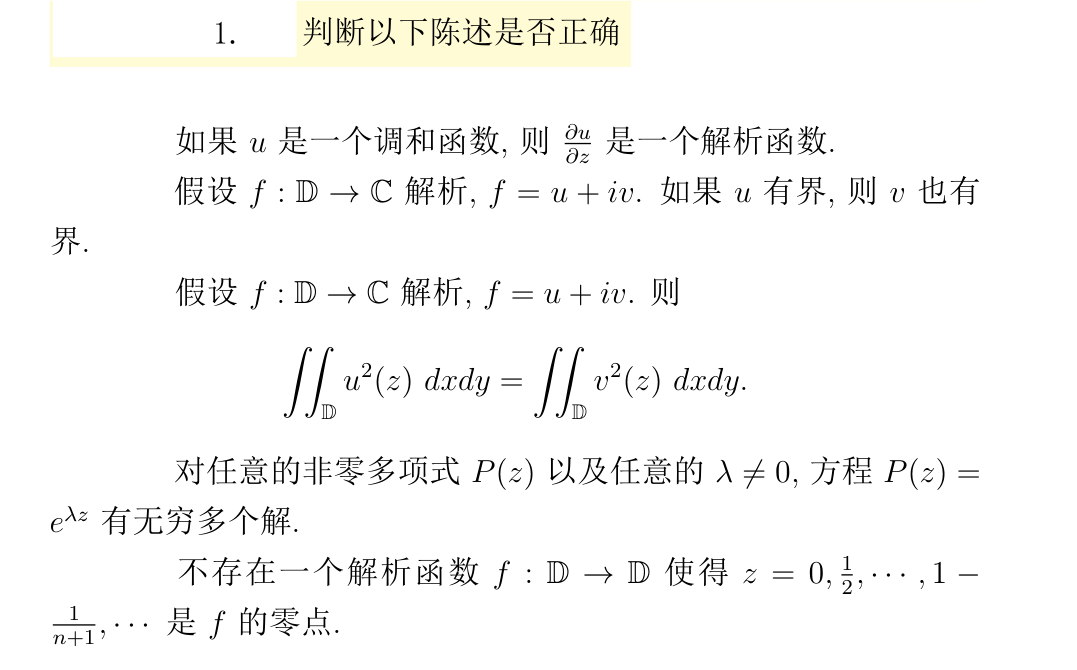
\includegraphics[width=\textwidth]{复变函数期末附加题-2025062123.png}
% \caption{}
\label{}
\end{figure}

\begin{enumerate}
	\item 对. $\partial_{\overline{z}}(\partial_{z}u)=\Delta u=0\Rightarrow \partial_{z}u\in H$.
	\item 错. 考虑 $f(z)\coloneqq\log(1-z)$.
	\item 错. $u^{2}-v^{2}=\text{Re }(f^{2})$. 由调和函数平均值公式得到,$LHS-RHS=\pi(\text{Re }f^{2}(0))$.
	\item 对. 考虑 $f(z)\coloneqq P(z)e^{ -\lambda z }$ 这是超越整函数,以 $\infty$ 为本性奇点,利用 Picard 大定理,在 $\infty$ 的任意邻域 $\{ \lvert z \rvert>R \}$ 内,除去至多一个点,$f$ 都可以取到任意值无穷多次. 由于 $P$ 为多项式,考虑不包含 $P$ 零点的 $\{ \lvert z \rvert\in R \}$,$f$ 取不到 0, 故除了 0 以外的任意值 (比如 1) 都可以取到无穷次.
	\item 对. 由于 $f\in N$,根据 Rudin theorem 15.23, $\sum_{n=1}^{\infty}(1-\lvert \alpha _n \rvert)<\infty$,即 $\sum_{n=1}^{\infty}\frac{1}{n}<\infty$,矛盾!
\end{enumerate}

\section{期末练习题}

\begin{figure}[H]
\centering
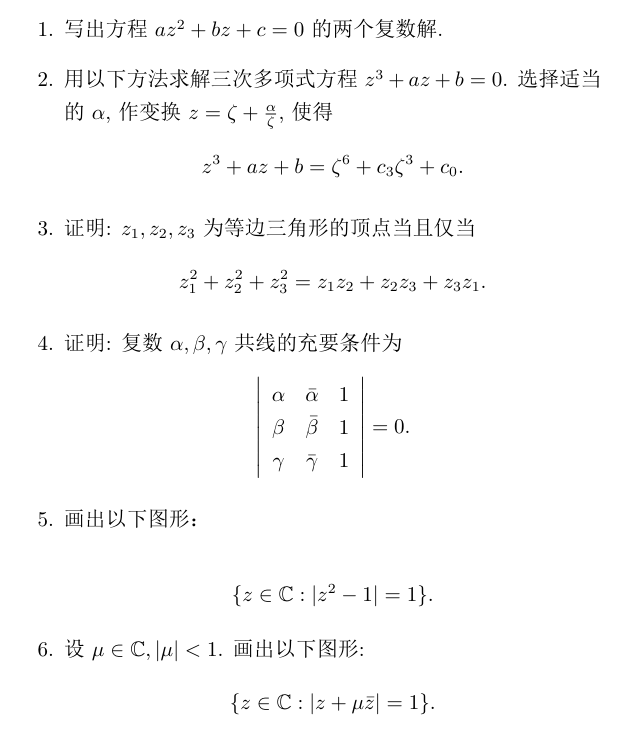
\includegraphics[width=\textwidth]{复变函数期末附加题-2025062319.png}
% \caption{}
\label{}
\end{figure}

\begin{enumerate}
	\item 略
	\item 略
	\item 等式成立当且仅当 $(z_1-z_2)^{2}+(z_2-z_3)^{2}+(z_3-z_1)^{2}=0$, 故可以不妨平移设 $z_1=0$,不妨伸缩旋转设 $z_2=1$,故显然.
	\item 不妨设 $a,b,c$ 非零,不妨设 $\alpha=1$,则必要性显然,充分性也显然.
	\item 考虑卡西尼卵
	\item $\mu\coloneqq a+bi$, then $x^2\left(1+a^2+b^2+2 a\right)+y^2\left(1+a^2+b^2-2 a\right)+4 b x y=1$.
\end{enumerate}

好的,\underline{卡西尼卵形线} (Cassini Oval) 是一个有趣的几何图形,它有许多独特的性质。以下是其主要性质的列举:

\begin{definition}
\textbf{卡西尼卵形线}是平面上所有满足到两个固定点(称为焦点 $F_1$ 和 $F_2$)的距离之乘积为常数 $k^2$ 的点的轨迹。如果点的坐标是 $(x, y)$,焦点是 $(-c, 0)$ 和 $(c, 0)$,则其定义方程为:
\[
\sqrt{(x+c)^2 + y^2} \cdot \sqrt{(x-c)^2 + y^2} = k^2
\]展开后可得到笛卡尔坐标方程:
\[
(x^2 + y^2)^2 - 2c^2(x^2 - y^2) + c^4 = k^4
\]或极坐标方程:
\[
r^4 - 2c^2 r^2 \cos(2\theta) + c^4 = k^4
\]
\end{definition}
卡西尼卵形线的形状非常多样,取决于常数 $k$ 与焦点半距离 $c$ 的关系:

\begin{enumerate}
	\item $k > c$ (单瓣卵形):
曲线是一个单个的闭合回路,形状像一个压扁的椭圆,包含两个焦点。随着 $k$ 的增大,它会变得越来越圆,当 $k \to \infty$ 时,趋近于一个以原点为圆心的大圆。
	\item $k = c$ (伯努利双纽线 / Lemniscate of Bernoulli):
曲线是一个形如“8”字或无限符号($\infty$)的图形,在原点处自相交。这是卡西尼卵形线的一个特殊且著名的形式,它与抛物线的反演有关。
	\item $k < c$ (双瓣卵形 / 两个分离的卵形):
曲线由两个分离的闭合回路组成,每个回路围绕一个焦点。随着 $k$ 减小,这两个卵形会变得越来越小,并趋近于焦点本身。
\end{enumerate}

卡西尼卵形线是关于 $x$ 轴和 $y$ 轴对称的。它也是关于原点(两个焦点的中点)中心对称的。

特殊点:

\begin{itemize}
	\item 交点:
卵形线可能与坐标轴有交点。例如,当 $y=0$ 时,方程变为 $(x^2-c^2)^2 = k^4$,解得 $x^2 = c^2 \pm k^2$,因此 $x = \pm\sqrt{c^2 \pm k^2}$。
	\item 焦点:
当 $k=c$ 时,曲线通过原点(两焦点的中点)。
\end{itemize}

与椭圆和双曲线的关系:

\begin{itemize}
	\item \textbf{椭圆} 定义为到两焦点的距离之\textbf{和}为常数。
	\item \textbf{双曲线} 定义为到两焦点的距离之\textbf{差的绝对值}为常数。
	\item \textbf{卡西尼卵形线} 定义为到两焦点的距离之\textbf{乘积}为常数。
\end{itemize}

它们都是圆锥曲线的推广,尽管卡西尼卵形线本身不是圆锥曲线。

反演性质:

伯努利双纽线 ($k=c$) 可以通过对一个双曲线进行反演(反转)来生成。或者说,对一个圆进行反演,可以得到一个双纽线。

应用:

\begin{itemize}
	\item 在物理学中,卡西尼卵形线出现在某些力场(如电荷或质量分布)的等势线中。
	\item 在光学中,它们可以用来描述某些透镜的表面。
	\item 在数学研究中,它们是代数几何和复分析中的一个经典例子。
\end{itemize}

极值点:

卡西尼卵形线的曲率、最大/最小宽度等性质可以通过分析其方程的导数来确定。

总之,卡西尼卵形线是一个因其定义方式(距离乘积)而产生的丰富多样的曲线族,其形状随参数变化而呈现出显著的差异。

\begin{figure}[H]
\centering
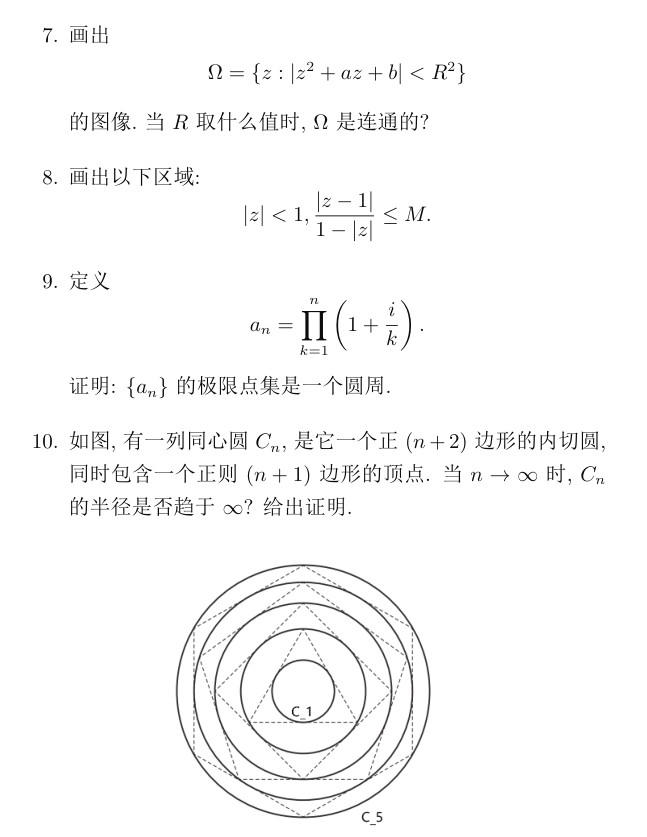
\includegraphics[width=\textwidth]{1-复变函数期末附加题-2025062319.png}
% \caption{}
\label{}
\end{figure}

\begin{enumerate}
	\item When $\lvert z_1-z_2 \rvert>2R$, i.e. $\left\lvert  \sqrt{ a^{2}-4b }  \right\rvert>R$.
	\item 是一个开圆盘,在 $M=1$ 时退化为 $[0,1)$,此外圆心在 $(-\infty,0)\cup(0,1)$.
	\item $\lvert a_n \rvert\leq \prod_{k=1}^{\infty}\sqrt{ 1+\frac{1}{k^{2}} }\leq \exp \left\{  \frac{1}{2}\sum_{k=1}^{\infty}\log(1+k^{-2})  \right\}\leq \exp \left\{  \frac{1}{2}\sum_{k=1}^{\infty}k^{-2}  \right\}<\infty$. And $\arg a_n=\sum_{k=1}^{n}\arctan\frac{1}{k}\sim \sum k^{-1}\to \infty$, where $\arctan\frac{1}{k}\to 0$. More explicitly, we have $\sin (\pi z)=\pi z\prod_{k=1}^{\infty}\left( 1-\frac{z^{2}}{k^{2}} \right)$, then $\lim_{ n \to \infty }\lvert a_n \rvert=\lim_{ n \to \infty }\sqrt{ 1+\frac{1}{k^{2}} }=\sqrt{ \frac{\sin i\pi}{\pi i} }=\sqrt{ \frac{\sinh(\pi)}{\pi} }$.
	\item $r_{n+1}\cos\frac{\pi}{n+2}=r_n$. Then
\[
\begin{aligned}
r_n=r_1\prod_{k=2}^{n}\frac{1}{\cos \frac{\pi}{k+1}} & =r_1\cdot\exp \left\{  -\sum_{k=2}^{n}\log \cos\frac{\pi}{k+1}  \right\} \\
 & =r_1\cdot \exp \left\{  -\sum_{k=2}^{n}\log\left( 1-\frac{1}{2}\left( \frac{\pi}{k+1} \right)^{2} +o(k^{-3})\right)  \right\} \\
 & =r_1\cdot \exp \left\{  -\sum_{k=2}^{n} \left( -\frac{1}{2} \right)\left( \frac{\pi}{k+1} \right)^{2}+o(1)  \right\} \\
 & < \infty
\end{aligned}
\]
\begin{figure}[H]
\centering
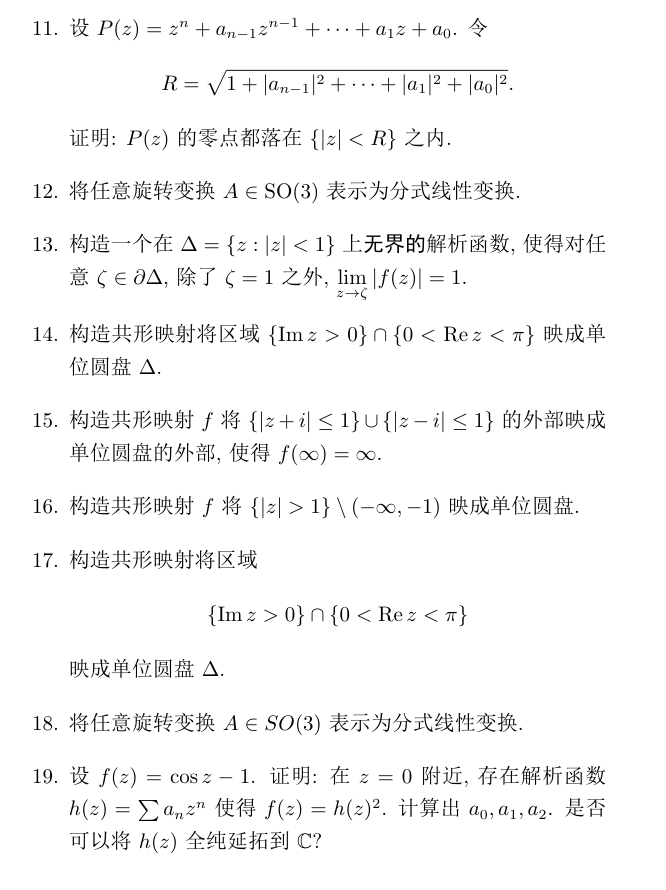
\includegraphics[width=\textwidth]{复变函数期末附加题-2025062320.png}
% \caption{}
\label{}
\end{figure}
	\item 这个不需要 Rouche 引理. 考虑 $P(z)=0$,有 $\lvert z \rvert ^{2n}\leq (\lvert a_{n-1} \rvert \lvert z \rvert ^{n-1}+\dots+\lvert a_0 \rvert)^{2}$,由 Cauchy-Schwarz,$RHS\leq \left( \lvert a_{n-1} \rvert ^{2}+\dots+\lvert a_0 \rvert ^{2} \right)(\lvert z \rvert ^{2n-2}+\dots+1)=(\lvert a_{n-1} \rvert ^{2}+\dots+\lvert a_0 \rvert ^{2})\frac{\lvert z \rvert ^{2n}-1}{\lvert z \rvert ^{2}-1}<(R^{2}-1)\frac{\lvert z \rvert ^{2n}}{\lvert z \rvert ^{2}-1}$ 于是 $\lvert z \rvert<R$.
	\item 任意一个旋转变换 $A \in \mathrm{SO}(3)$ 都可以通过以下步骤表示为一个分式线性变换:
1. 找到与旋转 $A$ 对应的 $\operatorname{SU}(2)$ 矩阵 $U=\left(\begin{array}{cc}\alpha & \beta \\ -\bar{\beta} & \bar{\alpha}\end{array}\right)$ 。
2. 这个矩阵 $U$ 定义了在黎最球面上的一个分式线性变换 $f_A(w)=\frac{\alpha w+\beta}{-\bar{\beta} w+\bar{\alpha}}$ 。
其中 $w$ 是旋转前点在黎最球面上的坐标,$w^{\prime}$ 是旋转后点在黎最球面上的坐标。这个表示是李群论和复变函数论之间的一个重要联系。
	\item 考虑 $w=\frac{1+z}{1-z}$,在 $z\neq1$ 的圆周上,这是个纯虚数 $w=-i\cot(\arg z/2 )$.
	\item $z_1:\Omega\to \{ \lvert z \rvert<1,\text{Im }z>0 \},z\mapsto e^{ iz }$, $z_2:\{ \lvert z \rvert<1,\text{Im }z>0 \}\to \{ \text{Im }z>0 \},z\mapsto-\frac{1}{2}\left( z+\frac{1}{z} \right)$, $z_3:\{ \text{Im }z>0 \}\to \{ \lvert z \rvert<1 \},z\mapsto\frac{z-i}{z+i}$.
	\item $z_1:\Omega\to \{ \lvert z \rvert>1 ,\text{Re }z>0\},z\mapsto -\sqrt{ z }$, $z_2:\{ \lvert z \rvert>1,\text{Re }z >0\}\to \{ \text{Re }z>0 \},z\mapsto\frac{1}{2}\left( z+\frac{1}{z} \right)$, $z_3:\{ \text{Re }z>0 \}\to \{ \lvert z \rvert>1 \},z\mapsto\frac{z+i}{z-i}$. 这个映射错了,没有满足 $f(\infty)=\infty$.
	\item 重复
	\item 重复
	\item 重复
	\item $\left[ \frac{f(z)}{z^{2}} \right]_{z=0}=-\frac{1}{2}$. 且 $\frac{f(z)}{z^{2}}$ 在 0 附近解析,故在 0 附近存在解析函数 $g(z)$ 使得 $\frac{f(z)}{z^{2}}=e^{ g(z) }$. 于是 $ze^{ g(z)/2 }\eqqcolon h(z)$. 我们知道 $h(z)=a_0+a_1z+a_2z^{2}+a_3z^{3}+\dots$,$f(z)=h^{2}(z)=a_0^{2}+2a_0a_1z+(a_1^{2}+2a_0a_2)z^{2}+(2a_0a_3+2a_1a_2)z^{3}+\dots$, 且 $f(z)$ 自己展开得到 $-\frac{1}{2}z^{2}+\frac{1}{24}z^{4}$. 故 $a_0=0$, $a_1^{2}=-\frac{1}{2}$, $a_1a_2=0$, 故 $a_1=\pm\frac{1}{\sqrt{ 2 }}i$, $a_2=0$.
\end{enumerate}

\begin{figure}[H]
\centering
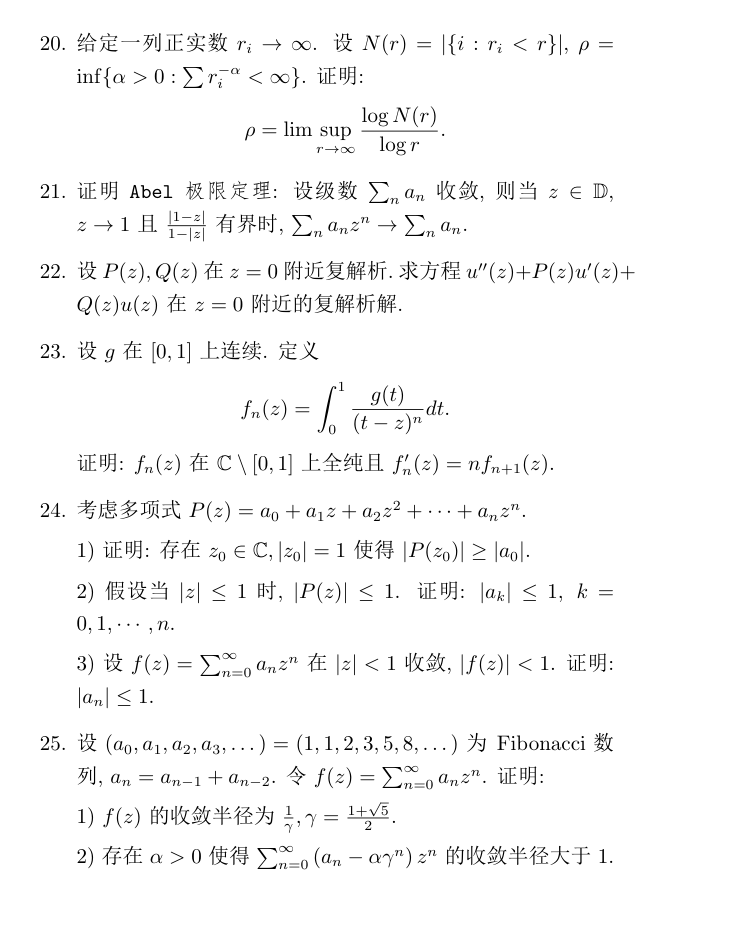
\includegraphics[width=\textwidth]{1-复变函数期末附加题-2025062320.png}
% \caption{}
\label{}
\end{figure}

\begin{figure}[H]
\centering
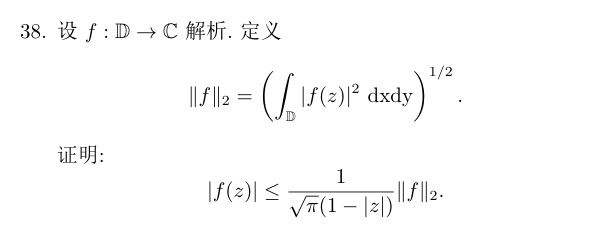
\includegraphics[width=\textwidth]{2-复变函数期末附加题-2025062320.png}
% \caption{}
\label{}
\end{figure}

由平均值公式,对于 $z\in \mathbb{D}$, $B_{r}(z)\subset \mathbb{D}$,有
\[
f(z)=\frac{1}{\pi r^{2}}\iint_{B_{r}(z)}f(\zeta)\,\mathrm{d}S  
\]
\[
\begin{aligned}
\iint_{B_{r}(z)}\lvert f(\zeta) \rvert \,\mathrm{d}S   & \leq \sqrt{ \iint_{B_{r}(z)}1\,\mathrm{d}S  \cdot\iint_{B_{r}(z)}\lvert f^{2}(\zeta) \rvert \,\mathrm{d}S  }  \\
 & =\sqrt{ \pi }r \cdot \lVert f \rVert _{2}
\end{aligned}
\]
于是
\[
\lvert f(z) \rvert \leq \frac{1}{\sqrt{ \pi }r}\lVert f \rVert _{2}
\]
令 $r\to1-\lvert z \rvert$,就有
\[
\lvert f(z) \rvert \leq \frac{1}{\sqrt{ \pi }(1-\lvert z \rvert )}\lVert f \rVert _{2}
\]
\begin{figure}[H]
\centering
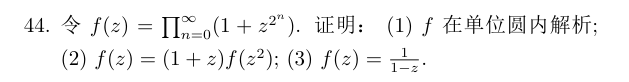
\includegraphics[width=\textwidth]{3-复变函数期末附加题-2025062320.png}
% \caption{}
\label{}
\end{figure}

\begin{enumerate}
	\item 在 $\lvert z \rvert\leq r<1$ 内,$\lvert f(z) \rvert\leq \exp \left\{  \sum_{n=0}^{\infty}\log(1+\lvert z \rvert ^{2^{n}})  \right\}\leq \exp \{ 1/(1-r) \}<\infty$,一致收敛,故解析. (思考 why)
	\item 显然
	\item $f(z)=(1+z)f(z^{2})=\dots=(1+z)\dots(1+z^{2^{N-1}})f(z^{2^{N}})=\frac{1-z^{2^{N}}}{1-z}\cdot f(z^{2^{N}})\to\frac{1}{1-z}f(0)=\frac{1}{1-z}$.
\end{enumerate}

\begin{figure}[H]
\centering
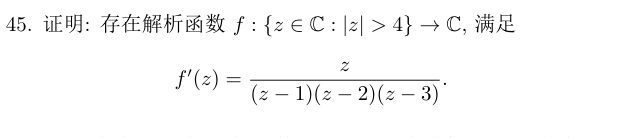
\includegraphics[width=\textwidth]{复变函数期末附加题-2025062321.png}
% \caption{}
\label{}
\end{figure}

记 $g=\frac{z}{(z-1)(z-2)(z-3)}$,于是计算得到 $\mathrm{res}_{\infty}g=-\mathrm{res}_{1}g-\mathrm{res}_{2}g-\mathrm{res}_{3}g=0$. 于是 $g$ 在 $\{ \lvert z \rvert>4 \}$ 内解析,可以良好定义 $f(z)=\int_{z_0\to z}^{} g(z) \, \mathrm{d}z$,其中 $\lvert z_0 \rvert>4$.

\begin{figure}[H]
\centering
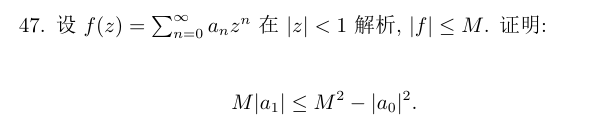
\includegraphics[width=\textwidth]{1-复变函数期末附加题-2025062321.png}
% \caption{}
\label{}
\end{figure}

不妨设 $M=1$ 否则用 $\frac{f}{M}$ 代替 $f$.

利用 Schwarz-pick 引理,$\varphi_{a}(z)\coloneqq\frac{z-a}{1-\overline{a}z}$. $g(z)\coloneqq\varphi_{f(\alpha)}\circ f\circ\varphi_{-\alpha}(z)$,于是
\[
\begin{aligned}
\lvert g'(0) \rvert &  =\lvert \varphi'_{f(\alpha)}(f(\varphi_{-\alpha}(0)))f'(\varphi_{-\alpha}(0))\varphi'_{-\alpha}(0) \rvert  \\
 & =\lvert \varphi'_{f(\alpha)}(f(\alpha))\cdot f'(\alpha)\cdot \varphi'_{-\alpha}(0)  \rvert \\
 & =\lvert 1-\lvert f(\alpha) \rvert ^{2}\rvert^{-1}   \cdot\lvert  f'(\alpha) \rvert \cdot\lvert 1-\lvert \alpha \rvert ^{2} \rvert  \\
 & \leq 1 
\end{aligned} 
\]
从而
\[
\lvert f'(\alpha) \rvert\leq \frac{1-\lvert f(\alpha) \rvert ^{2}}{1-\lvert \alpha \rvert ^{2}}
\]
令 $\alpha=0$ 就有
\[
\lvert f'(0) \rvert \leq 1-\lvert f(0) \rvert ^{2}
\]
\begin{figure}[H]
\centering
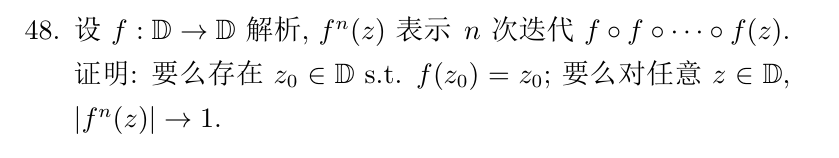
\includegraphics[width=\textwidth]{复变函数期末附加题-2025062522.png}
% \caption{}
\label{}
\end{figure}

This is Denjoy-Wolff theorem.

\begin{exercise}
\begin{figure}[H]
\centering
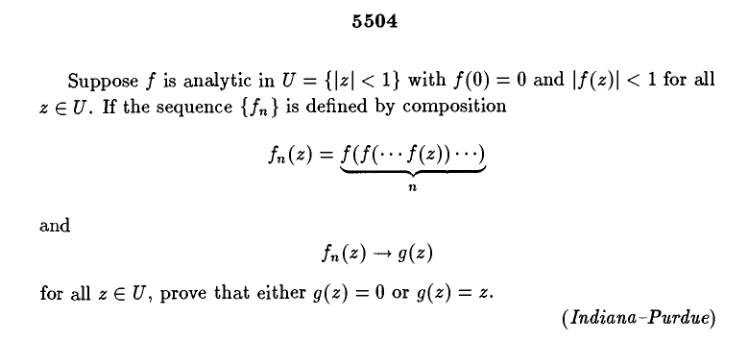
\includegraphics[width=\textwidth]{1-复变函数期末附加题-2025062522.png}
% \caption{}
\label{}
\end{figure}
\end{exercise}
\begin{figure}[H]
\centering
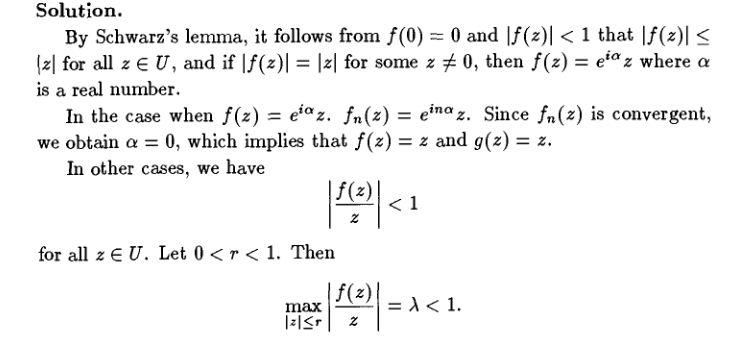
\includegraphics[width=\textwidth]{2-复变函数期末附加题-2025062522.png}
% \caption{}
\label{}
\end{figure}
\begin{figure}[H]
\centering
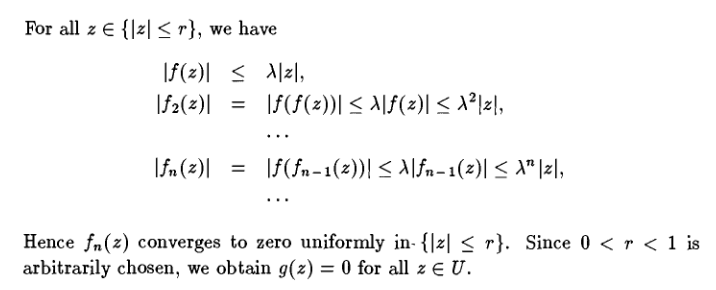
\includegraphics[width=\textwidth]{3-复变函数期末附加题-2025062522.png}
% \caption{}
\label{}
\end{figure}

\begin{figure}[H]
\centering
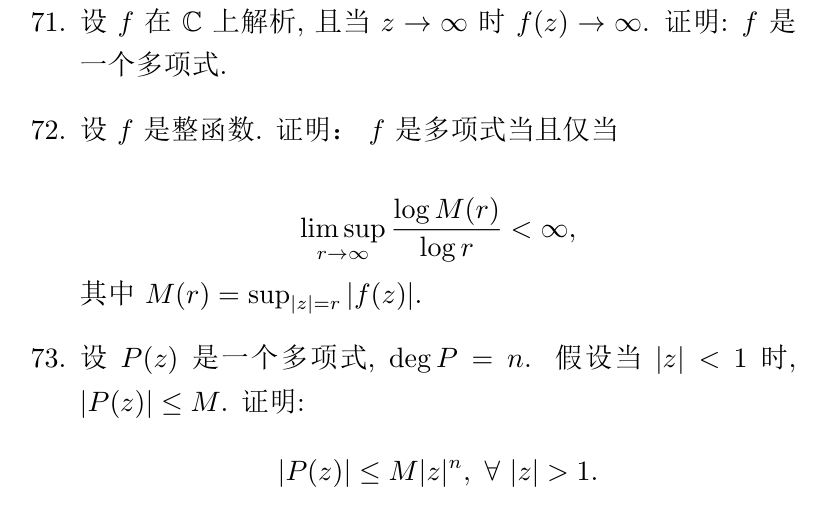
\includegraphics[width=\textwidth]{复变函数期末附加题-2025062523.png}
% \caption{}
\label{}
\end{figure}

\begin{itemize}
	\item 	\begin{enumerate}
		\item $g(z)\coloneqq f\left( \frac{1}{z} \right)$, 在 0 处有奇点,若为本性奇点,则由 Picard 大定理,$g$ 在 0 去心邻域内,除一个值以外,取到任意值无穷次,但 $\lim_{ z \to 0}g(z)=\infty$. 故 0 为极点,$g(z)=c_{-n}z^{-n}+\dots+c_0+c_1z+\dots$, 于是 $f(z)=\dots+c_1z^{-1}+c_0+c_{-1}z+\dots+c_{-n}z^{n}$,由于 $f\in H(\mathbb{C})$,$f$ 不可能在 0 处存在奇点,所以 $f(z)=c_0+c_{-1}z+\dots+c_{-n}z^{n}$ 是多项式.
	\end{enumerate}
	\item 	\begin{enumerate}
		\item 使用 Cauchy 积分公式放缩
	\end{enumerate}
	\item 	\begin{enumerate}
		\item 利用最大模原理,考虑解析函数 $Q (z)\coloneqq z^{n}P\left( \frac{1}{z} \right)$,对于 $\lvert z \rvert=1$,有 $\lvert Q(z) \rvert=\left\lvert  z^{n}P\left( \frac{1}{z} \right)  \right\rvert=\left\lvert  P\left( \frac{1}{z} \right)  \right\rvert\leq M$,这利用了 $\left\lvert  \frac{1}{z}  \right\rvert=1$,以及 $P$ 的连续性. 由最大模原理,对于 $\lvert z \rvert>1$,$\left\lvert  \frac{1}{z^{n}}P(z)  \right\rvert=\left\lvert  Q\left( \frac{1}{z} \right)  \right\rvert\leq \max_{\left\lvert  \frac{1}{z}  \right\rvert=1}\left\lvert  Q\left( \frac{1}{z} \right)  \right\rvert=M$.
	\end{enumerate}
\end{itemize}

\begin{figure}[H]
\centering
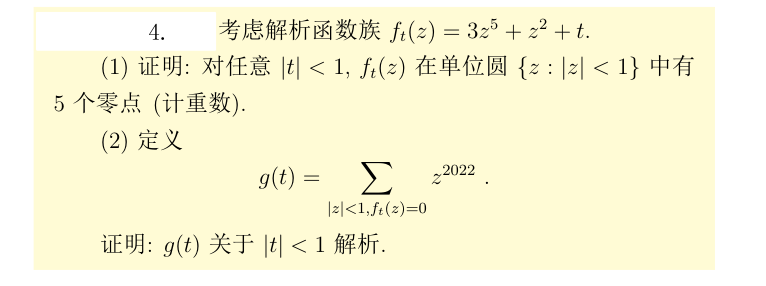
\includegraphics[width=\textwidth]{1-复变函数期末附加题-2025062600.png}
% \caption{}
\label{}
\end{figure}

Use the same idea as the Principle theorem.

$\{ z_j \}$ are the 5 distinct zero's of $f_{t}(z)$ in $\mathbb{D}$, $f_{t}(z)\coloneqq(z-z_j)h_{t}(z)$, then
\[
\frac{f'_{t}(z)}{f_{t}(z)}=\frac{1}{z-z_j}+\frac{h_{t}'(z)}{h_{t}(z)}
\]
So the residue of $\frac{f_{t}'(z)}{f_{t}(z)}$ at $z_j$ is 1. Thus for holomorphic $\phi(z)$,
\[
\mathrm{res}\left( \phi(z)\frac{f_{t}'(z)}{f_{t}(z)} ;z_j\right)=\phi(z_j)
\]
Then by residue theorem
\[
\int_{\lvert z \rvert =1}^{} \phi(z)\frac{f_{t}'(z)}{f_{t}(z)} \, \mathrm{d}z=2\pi i\sum_{j}\mathrm{res} \left( \phi(z)\frac{f_{t}'(z)}{f_{t}(z)};z_j \right)=2\pi i \sum_{j}\phi(z_j)
\]
Then
\[
g(t)=\sum \phi(z_j)=\frac{1}{2\pi i}\int_{\lvert z \rvert =1}^{}\phi(z)\frac{f_{t}'(z)}{f_{t}(z)}  \, \mathrm{d}z 
\]
\begin{figure}[H]
\centering
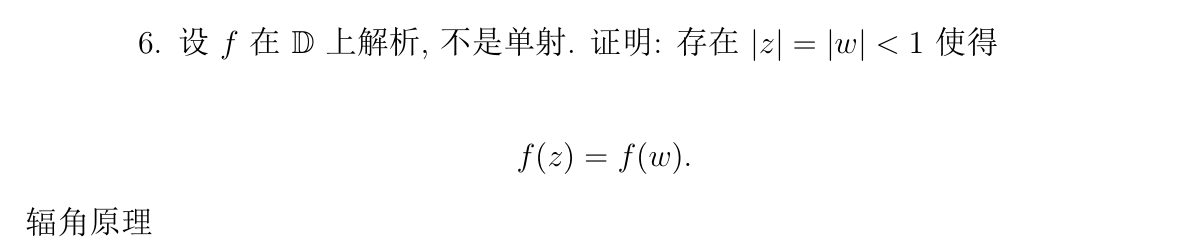
\includegraphics[width=\textwidth]{复变函数期末附加题-2025062600.png}
% \caption{}
\label{}
\end{figure}

假如对于任意满足 $f(z)=f(w)$ 的 $z,w$ 都有 $\lvert z \rvert<\lvert w \rvert=r$,由于 $z\in \mathbb{D}_{\lvert z \rvert}$,所以 $f (z)\in f(\mathbb{D}_{\lvert z \rvert})\subset f(\mathbb{D}_{r})$ ,同时 $f (z)=f (w)\in f(\partial \mathbb{D}_{r})=\partial f(\mathbb{D}_{r})$,由开映射定理 $f(\mathbb{D}_{r})$ 开,故矛盾!
